\subsection{Dafny Features}

\subsubsection{Counter Examples}
A useful features which also can provide a huge benefit, is to show an example which violates the contract, if the program can't be verified. Especially if the method is large with many branches, it can be very difficult to see how an example could look like, which is not correct regarding the contract. \newline
Z3 verifies mathematical expression by trying to find a proof for the negation of the proof. That means if it finds a proof the program is not correct. But more important Z3 finds a assignment for the different variables which violates the contract. This knowledge can be used to show a counterexample in Visual Studio Code. The only big step is to translate the counterexample, which is called model in Z3, back into something that can be matched with the Dafny program. Fortunately this is already done in the DafnyProvider in Boogie. Additionally to get only the necessary information out of it and also to show the values of class fields the translation needed to be extended. At the end a new verb counterExample was introduced, which returns a counter example json encoded. Thereby it was possible to show assignments of the variables on each line in Visual Studio Code. \newline
This is a easy example of a invalid method which should return the ABS, but misses to handle negative numbers correctly. 
\begin{figure}[H]
	\centering
	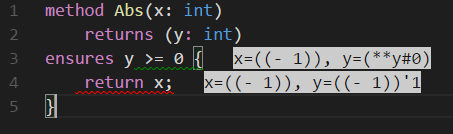
\includegraphics[width=1\textwidth]{img/counterModel}
	\caption{CounterExample is shown in Visual Studio Code}
	\label{fig:counterModel}
\end{figure}

Below is a more complex example of a class. The goal of the withdraw method is to prevent the balance to be below zero. Therefore the postcondition "ensures balance >= 0" exists. With help of the countermodel it becomes clear, that the amount is to big. It is bigger than zero though, but this precondition is wrong. It should be that the balance must be smaller than balance. On the first line it shows, that the balance is 2275 and the amount 2276. This results that the balance is after the subtraction negative. 
\begin{figure}[H]
	\centering
	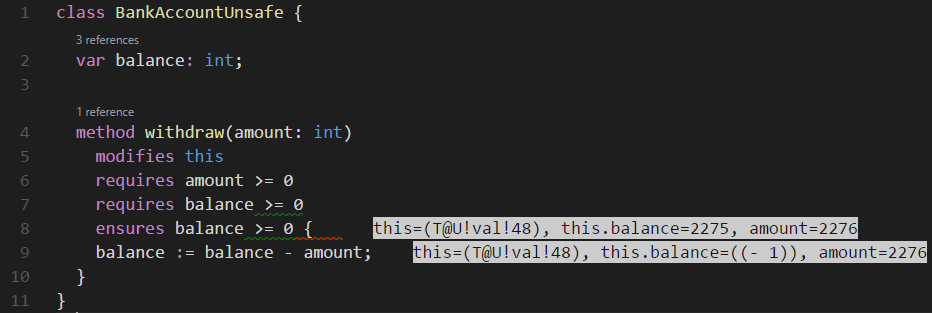
\includegraphics[width=1\textwidth]{img/counterModelBank}
	\caption{CounterExample inside a class}
	\label{fig:counterModelBank}
\end{figure}



\subsubsection{Quick Fixes} \label{quickfixes}
Quick Fixes are a versatile feature in IDEs which basically allow to do any manipulation to code. Usually they are offered as reactions to diagnostics which were provided earlier. A simple example would be implementing a spell checker this way, offering to replace a wrongly written word with the correct spelling. \newline
Since this feature has no clear implementation guideline, and the plugin designer can implement almost anything that he likes this way, this was an obvious place to implement Dafny specific feature in the plugin. A deeper insight why the following features were chosen can be found in \ref{addCodeActions}. \newline
They way this works in Visual Studio Code is that when the diagnostic stage for the file has been completed, where all things such as compiler warnings or custom warnings are generated, a new request is fired at the language server. This request holds a collection of all diagnostics on the current file and the the language server is free to either do nothing are provide commands for some diagnostics in the collection which often aim to resolve the shortcomings detailed by the diagnostic. \newline
\begin{figure}[H]
	\centering
	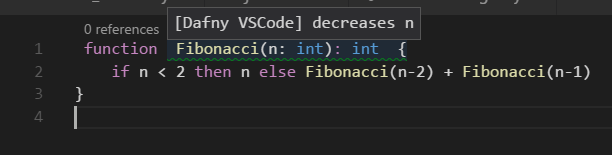
\includegraphics[width=0.7\textwidth]{img/diagnostic}
	\caption{Visual Studio Code displays a diagnostic}
	\label{fig:diagnostic}
\end{figure}
The current stand of the projects offers three code fixes to resolve Dafny specific diagnostics. \newline
The first one is a common situation where a programmer fails to capture his intention that an expression should either decrease or increase when working with recursion or loops. It can also be the case that an expression must always evaluate into a certain range, this is for instance the case when an expression that is used as an index to an array is not constant within a loop. The remedy is simple, a decrease / increase guard with the expression in question must be added at the correct location. In case an expression must be within a certain range, the same intent can be written as an invariant. \newline
\begin{figure}[H]
	\centering
	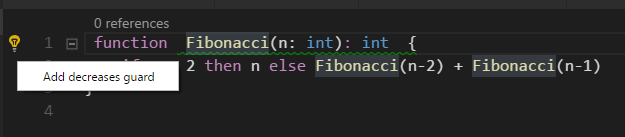
\includegraphics[width=0.7\textwidth]{img/decreaseGuard}
	\caption{Offering a code fix to add a guard}
	\label{fig:decreaseguard}
\end{figure}
This situation can easily be identified through the message within the diagnostic, since Dafny always gives this message in the same format. The expression that has to be decreased can also easily be parsed out of this message. The placement of the guard is a little more difficult, the implementation tries to find the first block in which the variable is not in scope anymore. The guard is then inserted before the block containing the first usage. \newline
\begin{figure}[H]
	\centering
	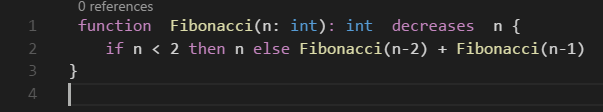
\includegraphics[width=0.7\textwidth]{img/decreaseGuardApplied}
	\caption{Program after the code fix}
	\label{fig:decreaseguardapplied}
\end{figure}
The second code fix the plugin offers is very similar, but this time the constraint is that an object may be null when it should not. The situation again is easily detected through the message in the diagnostic, and also the expression which should not be null can be parsed through it.
\begin{figure}[H]
	\centering
	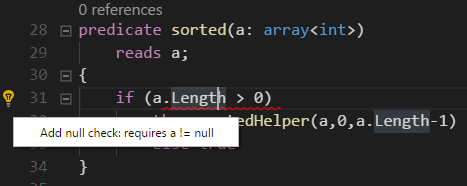
\includegraphics[width=0.7\textwidth]{img/nullCheck}
	\caption{It should be made sure that an element is not null}
	\label{fig:nullcheck}
\end{figure}
Also the search for the insertion position works very similarly. It then inserts the constraint in form of a precondition to the surrounding element. \newline
\begin{figure}[H]
	\centering
	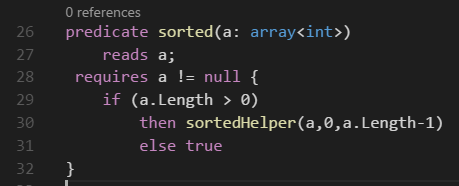
\includegraphics[width=0.7\textwidth]{img/nullCheckApplied}
	\caption{The precondition has been added}
	\label{fig:nullcheckapplied}
\end{figure}
The third code fix is to implement bound checking for expression which are used to index an array. This can either take the form of a precondition, if the expression is constant within the block of code in question, are the form of an invariant if the expression is dynamic (for instance in a loop).
The remedy is to apply the bound checking either through preconditions or invariants, depending on the context.
\begin{figure}[H]
	\centering
	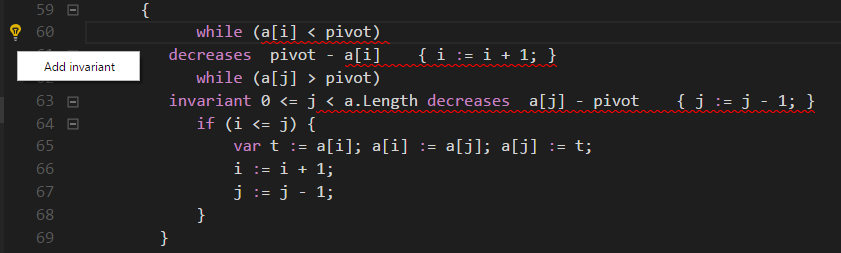
\includegraphics[width=1\textwidth]{img/indexOutRangeDiag}
	\caption{The expression may be out of range}
	\label{fig:indexOutOfRange}
\end{figure}
The first difficult part is to find the expression that is used as an index, as well as the identifier which stands for the array. Both is done through pattern matching on the code file in regard to the position of the diagnostic. Next it must be decided if preconditions or invariants should get generated, for this there must be knowledge about the context, e.g. if the expression is static through in the current block. This is done via the information saved in the symbol service and also some pattern matching. \newline
Finally, the invariant or the preconditions must be inserted into the correct place. For this, all identifiers used in the expressions must be matched against their declaration, in order place the guards when already all symbols are declared. \newline
\begin{figure}[H]
	\centering
	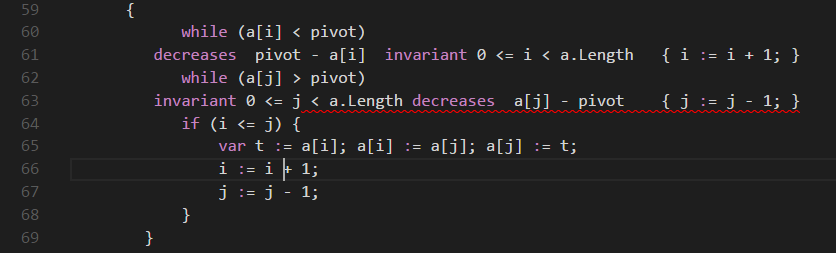
\includegraphics[width=1\textwidth]{img/indexChecked}
	\caption{Invariants for the loop were generated}
	\label{fig:indexInBound}
\end{figure}
At the current stand, only these three code fixes are implemented, the possible extensions are legion. One idea is to insert code that decreases a given expression when Dafny can't prove that an expression always decreases in a block were such a decrease clause was declared.\newline

